\chapter{Ergebnisse}
\label{chap:ergebnisse}

Dieses Kapitel wertet die Läufe des Double-DQN-Agenten (DDQN) aus Kapitel~\ref{chap:implementierung} unter dem Protokoll aus Kapitel~\ref{chap:evaluierung} aus. Trainiert wurde je Seed $s\in\{0,1,2\}$ mit 20\,000 Iterationen à 32 parallel erzeugten Flüssen, deren SNR pro Fluss zufällig aus $\{30,20,10,5\}$\,dB gezogen wurde. Die Bewertung erfolgt greedy ($\epsilon=0$) auf je 20\,000 frischen Flüssen pro SNR-Stufe. Alle Werte sind Mittelwerte über die drei Seeds, die Streuung ist als Standardabweichung $\sigma$ über die Seeds angegeben. Precision, Recall und F1-Score beziehen sich auf die Klasse DDoS.

\section{DDQN-Leistung über die SNR-Stufen}
\label{sec:ddqn_snr}

Tabelle~\ref{tab:ddqn_snr} fasst die Metriken des DDQN-Agenten zusammen, Abbildung~\ref{fig:snr_robustheit} zeigt denselben Verlauf mit Fehlerbalken von $\pm\sigma$.

\begin{table}[htbp]
	\centering
	\renewcommand{\arraystretch}{1.2}
	\caption{Precision, Recall und F1-Score des DDQN-Agenten je SNR-Stufe (Mittelwert $\pm$ Standardabweichung über drei Seeds, 20\,000 Testflüsse je Stufe).}
	\label{tab:ddqn_snr}
	\begin{tabular}{cccc}
		\toprule
		\textbf{SNR [dB]} & \textbf{Precision} & \textbf{Recall} & \textbf{F1-Score} \\
		\midrule
		30 & $0{,}8853 \pm 0{,}0021$ & $0{,}9018 \pm 0{,}0022$ & $0{,}8935 \pm 0{,}0009$ \\
		20 & $0{,}8813 \pm 0{,}0023$ & $0{,}8977 \pm 0{,}0015$ & $0{,}8894 \pm 0{,}0016$ \\
		10 & $0{,}8120 \pm 0{,}0048$ & $0{,}8485 \pm 0{,}0029$ & $0{,}8298 \pm 0{,}0037$ \\
		5  & $0{,}6963 \pm 0{,}0042$ & $0{,}7583 \pm 0{,}0031$ & $0{,}7260 \pm 0{,}0037$ \\
		\bottomrule
	\end{tabular}
\end{table}

\begin{figure}[htbp]
	\centering
	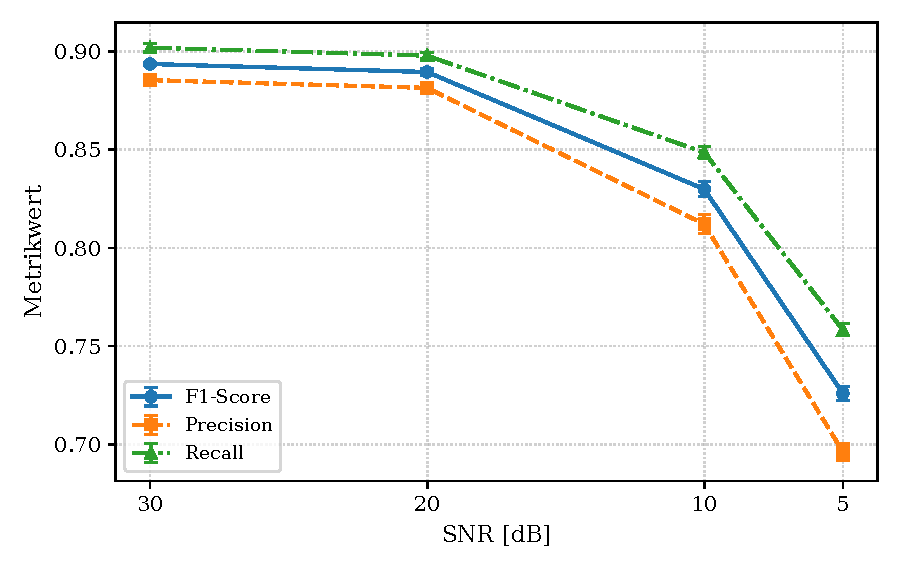
\includegraphics[width=0.85\textwidth]{snr_robustheit_plot.pdf}
	\caption{Precision, Recall und F1-Score des DDQN-Agenten über der SNR des AWGN-Kanals (30 bis 5\,dB). Marker: Mittelwert über drei Seeds, Fehlerbalken: $\pm$ eine Standardabweichung.}
	\label{fig:snr_robustheit}
\end{figure}

Der F1-Score fällt monoton von $0{,}8935$ bei 30\,dB über $0{,}8894$ (20\,dB) und $0{,}8298$ (10\,dB) auf $0{,}7260$ bei 5\,dB. Der Abfall verläuft nicht linear. Zwischen 30 und 20\,dB verliert der Agent nur $0{,}4$ Prozentpunkte, zwischen 10 und 5\,dB dagegen $10{,}4$. Das folgt aus dem Kanalmodell: Die Rauschvarianz je Merkmal beträgt $P_x/10^{\mathrm{SNR}/10}$, bei 30\,dB also $10^{-3}P_x$ und bei 5\,dB rund $0{,}32\,P_x$. Bei 20\,dB und darüber liegt die zusätzliche Varianz deutlich unter der intrinsischen Klassenstreuung von $\sigma=0{,}20$ je Merkmal und verändert die Überlappung der Klassen kaum. Bei 5\,dB überwiegt sie diese Streuung und verschmiert die Klassengrenze, die ohnehin nur über Mittelwertdifferenzen von $0{,}15$ bis $0{,}25$ je Merkmal definiert ist.

Die Streuung über die Seeds bleibt klein ($\sigma\le 0{,}0048$ bei allen Metriken) und wächst bei 10 und 5\,dB gegenüber 30\,dB auf das Zwei- bis Vierfache. Die Trainingsläufe konvergieren also reproduzierbar, bei starkem Rauschen reagiert die gelernte Entscheidungsgrenze jedoch empfindlicher auf die Initialisierung.

\subsection{Wirkung der asymmetrischen Reward-Funktion}
\label{sec:reward_recall}

Der Recall liegt auf allen vier SNR-Stufen über der Precision, am deutlichsten bei 5\,dB ($0{,}7583$ gegenüber $0{,}6963$). Das ist die direkte Folge der Belohnungsstruktur $R_{TP}=+1$, $R_{TN}=+0{,}5$, $R_{FP}=-1$, $R_{FN}=-2$. Da jeder Fluss eine Ein-Schritt-Episode ist, lernt die Q-Funktion den erwarteten Reward der Sofortentscheidung. Für die Angriffs-Posterior $p=P(\text{DDoS}\mid x)$ gilt
\begin{equation}
	Q(x,1)=p\cdot 1+(1-p)(-1)=2p-1,\qquad
	Q(x,0)=p\cdot(-2)+(1-p)\cdot 0{,}5=0{,}5-2{,}5\,p .
\end{equation}
Der Agent wählt \emph{DDoS}, sobald $Q(x,1)>Q(x,0)$ gilt, also für $p>1/3$. Ein symmetrisch bestrafender Klassifikator entscheidet dagegen bei $p>1/2$. Die Entscheidungsschwelle wandert damit zugunsten der Angriffsklasse. Der Agent akzeptiert mehr False Positives, um False Negatives zu vermeiden, und gibt Precision für Recall ab.

Das erklärt auch, warum bei sinkender SNR die Precision stärker einbricht als der Recall: Von 30 auf 5\,dB verliert die Precision $18{,}9$ Prozentpunkte, der Recall $14{,}4$. Mit zunehmender Unsicherheit der Posterior rutscht ein wachsender Anteil normaler Flüsse (Priorwahrscheinlichkeit $0{,}7$) über die abgesenkte Schwelle von $1/3$ und erzeugt zusätzliche Fehlalarme. Unter starkem Rauschen verhält sich der Agent konservativ im Sinne der Angriffserkennung, nicht im Sinne der Fehlalarmvermeidung.

\section{Vergleich mit klassischen Baselines}
\label{sec:baseline_vergleich}

Als Referenz dienen Random Forest (200 Bäume), SVM mit RBF-Kernel und ein MLP mit zwei verdeckten Schichten à 128 Neuronen. Sie verwenden dieselbe Datengenerierung und denselben AWGN-Kanal, dieselben Seeds und exakt dieselben Testflüsse je Seed und SNR-Stufe wie der DDQN. Trainiert wurden sie überwacht auf 20\,000 Flüssen mit pro Fluss gemischtem SNR. Tabelle~\ref{tab:f1_vergleich} stellt die F1-Scores gegenüber, Abbildung~\ref{fig:baseline_vergleich} zeigt den Verlauf.

\begin{table}[htbp]
	\centering
	\setlength{\tabcolsep}{4pt}
	\renewcommand{\arraystretch}{1.2}
	\caption{F1-Score von DDQN, Random Forest, SVM (RBF) und MLP je SNR-Stufe (Mittelwert $\pm$ Standardabweichung über drei Seeds). Fettdruck: höchster Mittelwert je Stufe.}
	\label{tab:f1_vergleich}
	\begin{tabular}{ccccc}
		\toprule
		\textbf{SNR [dB]} & \textbf{DDQN} & \textbf{Random Forest} & \textbf{SVM (RBF)} & \textbf{MLP} \\
		\midrule
		30 & $\mathbf{0{,}8935} \pm 0{,}0009$ & $0{,}8739 \pm 0{,}0032$ & $0{,}8857 \pm 0{,}0020$ & $0{,}8910 \pm 0{,}0010$ \\
		20 & $\mathbf{0{,}8894} \pm 0{,}0016$ & $0{,}8662 \pm 0{,}0026$ & $0{,}8795 \pm 0{,}0013$ & $0{,}8841 \pm 0{,}0022$ \\
		10 & $\mathbf{0{,}8298} \pm 0{,}0037$ & $0{,}8037 \pm 0{,}0031$ & $0{,}8211 \pm 0{,}0016$ & $0{,}8265 \pm 0{,}0064$ \\
		5  & $\mathbf{0{,}7260} \pm 0{,}0037$ & $0{,}6972 \pm 0{,}0060$ & $0{,}7097 \pm 0{,}0047$ & $0{,}7198 \pm 0{,}0003$ \\
		\bottomrule
	\end{tabular}
\end{table}

\begin{figure}[htbp]
	\centering
	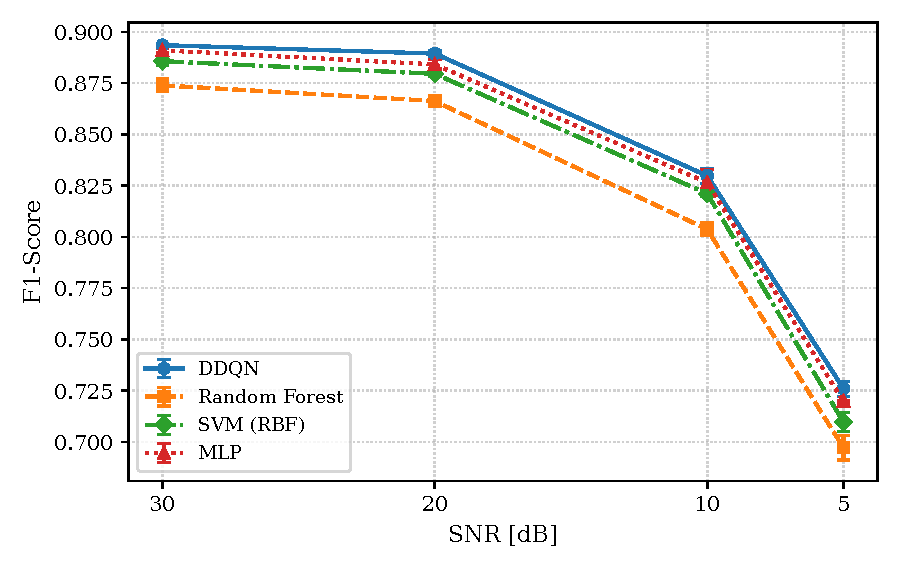
\includegraphics[width=0.85\textwidth]{baseline_vergleich_plot.pdf}
	\caption{F1-Score von DDQN, Random Forest, SVM (RBF) und MLP über der SNR des AWGN-Kanals. Marker: Mittelwert über drei Seeds, Fehlerbalken: $\pm$ eine Standardabweichung.}
	\label{fig:baseline_vergleich}
\end{figure}

Alle vier Verfahren zeigen denselben monotonen Abfall, und der DDQN erreicht auf jeder Stufe den höchsten mittleren F1-Score. Der Vorsprung ist allerdings klein. Gegenüber dem MLP, dem stärksten Baseline-Modell, beträgt er $0{,}25$ (30\,dB), $0{,}53$ (20\,dB), $0{,}33$ (10\,dB) und $0{,}62$ Prozentpunkte (5\,dB). Die SVM liegt zwischen $0{,}78$ und $1{,}63$, der Random Forest zwischen $1{,}96$ und $2{,}88$ Prozentpunkten zurück. Die Abstände zum MLP bewegen sich in der Größenordnung der Seed-Streuung, bei 10\,dB ($\sigma_{\mathrm{MLP}}=0{,}0064$) überlappen die Fehlerbalken. Mit drei Seeds lässt sich daraus keine statistische Signifikanz ableiten. Belastbar ist lediglich die Rangfolge DDQN $\gtrsim$ MLP $>$ SVM $>$ Random Forest, die auf allen vier Stufen identisch ausfällt.

Der DDQN erzielt seinen F1-Wert über einen anderen Arbeitspunkt als die Baselines. Beim Random Forest betragen Precision und Recall bei 30\,dB $0{,}9260$ und $0{,}8274$, beim DDQN $0{,}8853$ und $0{,}9018$. Die überwacht und ohne Kostengewichtung trainierten Baselines wählen die symmetrische Schwelle $p>1/2$ und landen entsprechend auf der Precision-Seite. Der F1-Score gewichtet beide Größen gleich und kann den Reward-getriebenen Arbeitspunkt des DDQN deshalb nur unvollständig bewerten. Unter der Kostenmatrix des Agenten, die einen verpassten Angriff doppelt so hoch bestraft wie einen Fehlalarm, fiele der Vorsprung gegenüber den Baselines voraussichtlich größer aus. Das wurde hier nicht gemessen.

Zwei Einschränkungen begrenzen die Aussagekraft des Vergleichs. Erstens sah der DDQN rund $6{,}4\cdot 10^{5}$ Trainingsflüsse (20\,000 Iterationen $\times$ 32), die Baselines nur $2\cdot 10^{4}$. Zweitens stammen alle Daten aus dem klassenbedingt gaußverteilten Generatormodell mit Angriffsanteil $0{,}3$. In einem solchen Modell erreicht schon ein kleines neuronales Netz eine nahezu Bayes-optimale Entscheidungsgrenze, was die geringen Unterschiede zwischen DDQN und MLP erklärt. Ob sich der Vorsprung auf realem Verkehr halten würde, bleibt offen.

\section{Robustheit nach RLA und ELA}
\label{sec:robustheit_rla_ela}

Tabelle~\ref{tab:rla_ela} wendet die Maße aus Abschnitt~\ref{sec:robustheitsmetriken} auf die mittleren F1-Scores an. Referenz ist jeweils die eigene Leistung des Modells bei 30\,dB.

\begin{table}[htbp]
	\centering
	\small
	\setlength{\tabcolsep}{4pt}
	\renewcommand{\arraystretch}{1.2}
	\caption{Relative Loss of Accuracy (RLA, in \%) und Equalized Loss of Accuracy (ELA) nach Sáez et al.\ \autocite{saezEvaluatingClassifierBehavior2016}, berechnet aus den mittleren F1-Scores über drei Seeds mit 30\,dB als Referenz. Kleinere Werte bedeuten höhere Robustheit.}
	\label{tab:rla_ela}
	\begin{tabular}{lccccccc}
		\toprule
		& \multicolumn{3}{c}{\textbf{RLA [\%]}} & \multicolumn{4}{c}{\textbf{ELA}} \\
		\cmidrule(lr){2-4}\cmidrule(lr){5-8}
		\textbf{Modell} & 20\,dB & 10\,dB & 5\,dB & 30\,dB & 20\,dB & 10\,dB & 5\,dB \\
		\midrule
		DDQN          & $\mathbf{0{,}46}$ & $\mathbf{7{,}13}$ & $\mathbf{18{,}75}$ & $\mathbf{0{,}119}$ & $\mathbf{0{,}124}$ & $\mathbf{0{,}191}$ & $\mathbf{0{,}307}$ \\
		MLP           & $0{,}77$ & $7{,}24$ & $19{,}21$ & $0{,}122$ & $0{,}130$ & $0{,}195$ & $0{,}315$ \\
		SVM (RBF)     & $0{,}70$ & $7{,}29$ & $19{,}87$ & $0{,}129$ & $0{,}136$ & $0{,}202$ & $0{,}328$ \\
		Random Forest & $0{,}88$ & $8{,}03$ & $20{,}22$ & $0{,}144$ & $0{,}153$ & $0{,}225$ & $0{,}347$ \\
		\bottomrule
	\end{tabular}
\end{table}

Die ELA ordnet die Modelle auf jeder Stufe gleich: DDQN vor MLP, SVM und Random Forest. Bei der RLA ist das nicht durchgehend so. Bei 20\,dB verliert die SVM relativ weniger als das MLP ($0{,}70$ gegenüber $0{,}77\,\%$), obwohl ihr F1-Score auf beiden Stufen niedriger liegt. Genau diesen Effekt korrigiert die ELA, indem sie den verbleibenden Fehler statt der Differenz bewertet.

Auffälliger als die Rangfolge ist die Spannweite. Bei 10\,dB liegen DDQN, MLP und SVM in der RLA nur $0{,}16$ Prozentpunkte auseinander, der Random Forest $0{,}9$ Prozentpunkte hinter dem DDQN. Bei 5\,dB verlieren alle vier Modelle zwischen $18{,}8$ und $20{,}2\,\%$ ihrer Ausgangsleistung. Der Großteil des Verlusts ist also nicht modellbedingt, sondern folgt aus der Klassenüberlappung des Kanals: Die Bayes-Fehlerwahrscheinlichkeit steigt im selben Intervall von $6{,}9$ auf $18{,}7\,\%$ (Tabelle~\ref{tab:klassenueberlappung}). Modellbedingt ist nur die Differenz zwischen den Verfahren, bei 5\,dB rund $1{,}5$ Prozentpunkte RLA zwischen DDQN und Random Forest. Wie beim F1-Vergleich gilt: Mit drei Seeds ist dieser Abstand nicht als signifikant nachgewiesen.

\section{Einordnung in die Literatur}
\label{sec:ergebnisse_literatur}

\paragraph{Random Forest als schwächste Baseline.} Arjoune et al. finden für die Jamming-Erkennung in der Accuracy die Rangfolge Random Forest ($96{,}6\,\%$) vor neuronalem Netz ($94{,}4\,\%$) und SVM \autocite{arjouneNovelJammingAttacks2020}. Hier fällt sie umgekehrt aus. Zwei Unterschiede erklären das. Bei Arjoune et al. ist die Kanalverschlechterung selbst das Ereignis, das die vier Linkqualitätsmerkmale (Bad Packet Ratio, Packet Delivery Ratio, Received Signal Strength, Clear Channel Assessment) anzeigen. Hier ist das Rauschen eine Störung, die alle acht Flussmerkmale überlagert und keine Information über die Klasse trägt. Der zweite Grund liegt im Generatormodell. Bei gleicher Kovarianz beider Klassen ist der Logarithmus des Likelihood-Verhältnisses linear in $\mathbf{y}$, die Bayes-optimale Grenze also eine Hyperebene mit der Normalen $\boldsymbol{\Sigma}^{-1}\Delta\boldsymbol{\mu}$. Weil $\boldsymbol{\Sigma}$ vom SNR abhängt, ändert sich ihre Richtung über die gemischten Trainingsstufen nur geringfügig, die Grenze bleibt nahezu linear und liegt schräg zu den Koordinatenachsen. Q-Netz, MLP und RBF-SVM bilden eine solche Fläche direkt ab. Ein Random Forest muss sie aus achsenparallelen Stufen zusammensetzen, und jede dieser Stufen reagiert auf Rauschen nahe ihrer Schwelle, wie es Zhu und Wu für Entscheidungsbäume beschreiben \autocite{zhuClassNoiseVs2004}.

\paragraph{DDQN und MLP.} Q-Netz und MLP haben dieselbe Struktur $8\to128\to128$ mit ReLU und unterscheiden sich im Lernziel. Das MLP schätzt über die Kreuzentropie die Posterior $p$ und entscheidet bei $p>1/2$. Das Q-Netz regressiert den erwarteten Reward und entscheidet damit bei $p>1/3$ (Abschnitt~\ref{sec:reward_recall}). Die fast gleichen ELA-Werte passen dazu: Beide lernen eine vergleichbar gute Repräsentation, der F1-Unterschied stammt überwiegend aus dem Arbeitspunkt. Zhang et al. zeigen, dass MLP-basierte NIDS unter gezielter Manipulation zeitbasierter Merkmale umgangen werden können \autocite{zhangAdversarialAttacksDeep2022}. Dieser Befund betrifft das Q-Netz gleichermaßen, da es architektonisch ein MLP ist.

\paragraph{Stochastische gegenüber gezielter Störung.} Die gemessene Robustheit gilt nur für AWGN. Merzouk et al. zeigen, dass die Accuracy eines DQN-Detektors unter FGSM von $84{,}81$ auf $66{,}87\,\%$ fällt \autocite{merzoukEvadingDeepReinforcement2022}. Der Unterschied lässt sich am Generatormodell abschätzen. In weißen Koordinaten, in denen die Klassenstreuung isotrop ist, entscheidet nur die Komponente der Störung entlang der Diskriminanten. Näherungsweise isotropes Rauschen legt im Mittel nur den Anteil $1/8$ seiner Leistung in diese Richtung, eine gezielte Störung ihre gesamte. Bei gleicher Leistung ist der gezielte Angriff damit um etwa den Faktor $\sqrt{8}\approx2{,}8$ in der Amplitude wirksamer. Ein gutes Ergebnis unter AWGN ist deshalb kein Beleg für adversariale Robustheit.

\section{Zusammenfassung}
\label{sec:ergebnisse_zusammenfassung}

Der DDQN-Agent erreicht bei 30\,dB einen F1-Score von $0{,}8935$ und hält bei 10\,dB noch $0{,}8298$. Bei 5\,dB fällt er auf $0{,}7260$. Der Recall übertrifft die Precision auf jeder Stufe, weil die Reward-Matrix die Entscheidungsschwelle von $p=1/2$ auf $p=1/3$ senkt. Gegenüber Random Forest, SVM und MLP liegt der DDQN auf allen vier SNR-Stufen vorn, der Abstand zum MLP bleibt jedoch unter einem Prozentpunkt und innerhalb weniger Standardabweichungen. Nach der ELA bleibt der DDQN auf allen Stufen das robusteste Verfahren ($0{,}307$ bei 5\,dB gegenüber $0{,}347$ beim Random Forest). Der größte Teil des Leistungsverlusts geht jedoch auf die wachsende Klassenüberlappung zurück und trifft alle Modelle ähnlich. Die Ergebnisse belegen die Robustheit des Ansatzes bis etwa 10\,dB, und zwar gegenüber stochastischem Rauschen, nicht gegenüber gezielten Angriffen. Einen klaren Überlegenheitsnachweis gegenüber überwacht trainierten Klassifikatoren liefern sie nicht.
